

\documentclass[aspectratio=169, 12pt]{beamer}

%%%%%%%%%%%%
% Packages %
%%%%%%%%%%%%

\usepackage{ctex}
\usepackage[english]{babel}
\usepackage{packages/sleek}
\usepackage{packages/tweaks}
\usepackage{calligra} % thanks pakeage

%%%%%%%%%%%%%%%%
% Bibliography %
%%%%%%%%%%%%%%%%

\addbibresource{./resources/bib/references.bib}

%%%%%%%%%%%%%%
% Title-page %
%%%%%%%%%%%%%%


\title{计量经济学}
\subtitle{Based on Metropolis theme}
\author[LIU ShHUAI]{刘 {  } 帅}
\institute{山西师范大学 {  } 经济与管理学院}
\date{\today}
\titlelogo{./resources/pdf/logo.png}
\framelogo{./resources/pdf/logo.png}

%%%%%%%%%%%%
% Document %
%%%%%%%%%%%%

\begin{document}

\maketitle

\begin{frame}[standout]
    案例分析一\par
    \addtolength{\parskip}{.4em}
    我国保障性住房制度的社会福利效应分析
\end{frame}

\begin{frame}[plain]
    % \begin{multicols}{1}
    %   \frametitle{Outline}
    %   \tableofcontents[hideallsubsections]
    % \end{multicols}
    \frametitle{Outline}
    \tableofcontents[hideallsubsections]
    % \tableofcontents[currentsection]
  \end{frame}

\section{内容提要}

\begin{frame}[plain]
    \frametitle{内容提要}
    近年来,我国保障性住房发展迅速,但由于建设速度过快,投入资金不足,
监管不严等原因,部分保障性住房存在分配不公、空置率过高、建筑质量差等问
题。\par
本文运用福利经济学理论,解释保障性住房制度的社会福利效应;分析保障
性住房由于建设环节的多主体利益博弈,分配环节的“寻租”、“随机分配”等
行为造成的社会福利损失。在借鉴国外先进经验的基础上,提出规范开发商行为
建立严格的准入、退出和监督机制,有效拓宽保障房源等完善保障性住房制度的
对策建议。
\end{frame}

\section{一、引言}

\begin{frame}{plain}
    \frametitle{保障性住房}
    保障性住房是与商品性住房相对应的概念,
    指政府为中低收入住房困难家庭提供的限定标准、限定价格或租金的住房。
    对于住房保障制度的社会福利效应,国外学者关注的是住房保障政策的效果。恩格斯把住房短缺归结为城市化、工业化快速发展的产物,政府对房地产市场的干预和管理具有必要性。
\end{frame}

\begin{frame}{plain}
    \frametitle{研究成果}
    20世纪90年代以来随着我国住房保障制度的建立和完善,
    相应的研究成果也日益丰富,主要包括三个方面:
    \begin{itemize}
        \item (1)保障房的供给方式。我国住房保障的供给方式主要有政府直接生产、政府给开发商提供补贴、政府对低收入人群发放补贴、政府对住房租金和价格实行管制等。
        \item (2)保障房的福利效应。现有研究运用模糊评价、帕累托最优、消费者剩余、动态博弈、效应函数等理论和方法,构建保障房福利效应评价指标体系,对我国城镇保障房的供给绩效进行了定量评价。
        \item (3)保障房建设的对策建议。
    \end{itemize}
\end{frame}

\begin{frame}[plain]
    \frametitle{现实问题}
    本案例针对我国保障房建设中暴露的“建设不佳,分配不公”等现实问题,利用福利经济学的相关理论,分析保障制度增进社会福利的基本原理,并对保障房建设过程中各行为主体利益博弈、分配过程中寻租行为给保障对象带来的社会福利损失进行评价,最后在借鉴发达国家先进经验的基础上提出完善我国保障房建设的对策建议。
\end{frame}

\section{二、我国保障性住房制度的社会福利增进效应}

\begin{frame}[plain]
    \frametitle{(一)住房分配失灵催生保障性住房制度}
    按照福利经济学第一原理在完全竞争市场条件下,通过市场配置住房资源可以实现帕累托最优,特别是依靠市场的住房分配在中高收入群体中是有效的;但是城镇中低收入群体、进城务工人员、新毕业大学生的住房需求难以得到满足,主要原因是在市场机制下,利润是厂商建设商品房的动力,在利润驱使下,低收入人群能够接受的低价格住房的有效供应不足。
\end{frame}

\begin{frame}[plain]
    \frametitle{(一)住房分配失灵催生保障性住房制度}
    在市场无法提供低收入人群能够接受的商品房前提下,按照福利经济学第二定理的理论解释,由政府提供保障性住房成为满足低收入人群住房需求的必然。首先,在市场经济环镜中的帕累托最优是理想状态,实际上市场供需与价格有关,隐藏着生产过剩的风险,若没有政府的干预,必将导致房地产市场的不稳定。其次,保障性住房具有资金规模要求大、投入周期长、资金不容易变现等特征,若该项资金由市场提供,会对企业造成很大负担,不利于企业的快速成长。
\end{frame}

\begin{frame}[plain]
    \frametitle{(二)保障性住房制度提升社会福利水平}
    从提供公共服务和收入再分配功能来看,政府主导的保障房制度属于对低收入群体进行收入再分配的福利政策,有利于促进低收入劳动者的人力资本积累和社会和谐,进而提升整个社会的福利水平。
\end{frame}

\begin{frame}[plain]
    \frametitle{(二)保障性住房制度提升社会福利水平}
    从福利经济学的角度保障房制度分配遵循帕累托改进原则,即在不使其他人情况变坏的情况下,使一些人情况变好,从而改进社会整体福利水平,以达到帕累托最优,中低收入群体以相对低廉的价格购买或租赁得到的住房,无论心里还是实际都使自身效用和利益得到满足和提升,而并不影响高收入群体的住房需求。从下图中可以看出低收入群体的福利改进。
\end{frame}

\begin{frame}[plain]
    \frametitle{(二)保障性住房制度提升社会福利水平}
    \begin{figure}[]
        \centering
        \begin{minipage}{0.4\linewidth}
            图中表示政府在住房市场上为低收入困难家庭提供保障房。设保障房的售价或租金水平为r1,而同类住房的市场售价或租金为r0,必有r1<r0;短期内,由于保障性住房的供给恒定不变,因而供给曲线s垂直于横轴,并于需求曲线d相交于点a。可知因为保障性住房的出现,产生消费者剩余eabf,这部分消费者剩余被低收入家庭无偿获得。
        \end{minipage}%
        \begin{minipage}{0.6\linewidth}
            \centering
            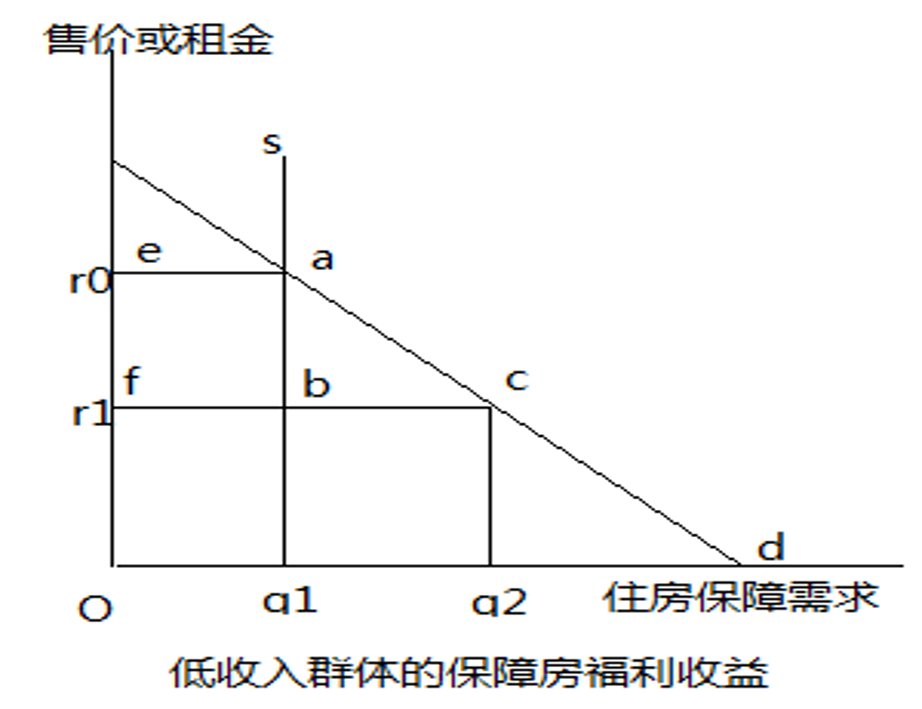
\includegraphics[width=1.0\textwidth]{./resources/figure/renthouse.png}
        \end{minipage}
        \end{figure}
\end{frame}

\section{三、我国保障性住房建设与分配中的社会福利损失}

\begin{frame}[plain]
    \frametitle{(一)保障性住房建设环节的社会福利损失}
    (1)开发商建设保障性住房的利润空间较低 \par
    我国《经济适用住房价格管理办法》明确规定经济适用房的利润率最高不得超过开发成本中排除管理费、贷款利息、行政事业性收费三项后余额的3\%。在同样投入了大量企业资源的情况下,从理性人的角度出发,开发商放弃百分之十几、百分之几十的利润率而选择建设保障房不是它们的最优选择。另一方面通过行政手段限定开发商利润率的做法,等于强行使开发商以利润损失为代价分摊政府应承担的住房保障职责。此外,开发保障房项目还可能对开发商的利益造成直接损害。
\end{frame}

\begin{frame}[plain]
    \frametitle{(一)保障性住房建设环节的社会福利损失}
    (2)地方政府缺乏保障房建设的内在动力\par
         导致地方政府缺乏保障房建设的内在动力主要表现在三个方面:\par
         a.在我国当前住房开发成本中,土地成本约占总成本的30\%,土地出让金是地方政府公共收入的主要来源之一。保障房制度正是通过地方政府免征土地出让金的方式实现对保障房开发商的补贴。该政策首先就触动了地方政府的利益,因此才会出现保障房的建设总量小、建设比例低,以及基于土地出让金的考虑,把保障房建设在城镇偏远区位的现象。
\end{frame}

\begin{frame}[plain]
    \frametitle{(一)保障性住房建设环节的社会福利损失}
    b.中央政府作为保障房政策的制定者,却没有为各地的保障房建设提供额外的财政补贴,完全由地方政府实施和承担费用,在中央和地方政府的职责分配上有失公平,降低了地方政府支持保障房政策的积极性。
    \par
    c.相对于购房者而言,地方政府与开发商在利益上更趋于一致。
\end{frame}

\begin{frame}[plain]
    \frametitle{(一)保障性住房建设环节的社会福利损失}
    (3)保障房建设数量不足导致社会福利损失\par
       由于政府和开发商建设保障房的积极性不足和内外动力缺失,使我国保障房的供应量远低于需求量,保障房政策实际发挥的作用有限。由此导致的保障房与商品房比例严重失调的现象,不仅加剧了城市居民的住房难问题,也制约了房地产业的健康发展。
\end{frame}

\begin{frame}[plain]
    \frametitle{(一)保障性住房建设环节的社会福利损失}
    开发商在利润的驱使下总是会使保障房变相化,购房者需要以比真实价格更高的价格和比不变相时更低的购买率来购买保障房,这是保障房制度设计下的博弈所造成的购房者福利损失。面对这一福利的损失,保障房的购房者因在博弈中处于弱势地位,无法改变福利受损现状;尽管他们可以选择不买,但不买就等于自动放弃该项政策提供的福利,收益降为零。
\end{frame}

\begin{frame}[plain]
    \frametitle{(一)保障性住房建设环节的社会福利损失}
    \begin{figure}
        \centering
        \begin{minipage}{0.4\linewidth}
            因此,保障房购房者往往在明知开发商的变相行为会使得自己利益受损的情况下也只能选择购买,已损失掉一部分本应属于自己的收益为代价换取剩余部分收益。若当开发商显性或隐性的改变保障房申购标准,一部分中高收入者便会加入到保障房的需求行列,使得一部分低收入者被挤出保障房购买者行列,引发保障房建设和购买中的挤出效应,如右图所示:
        \end{minipage}%
        \begin{minipage}{0.6\linewidth}
            \centering
            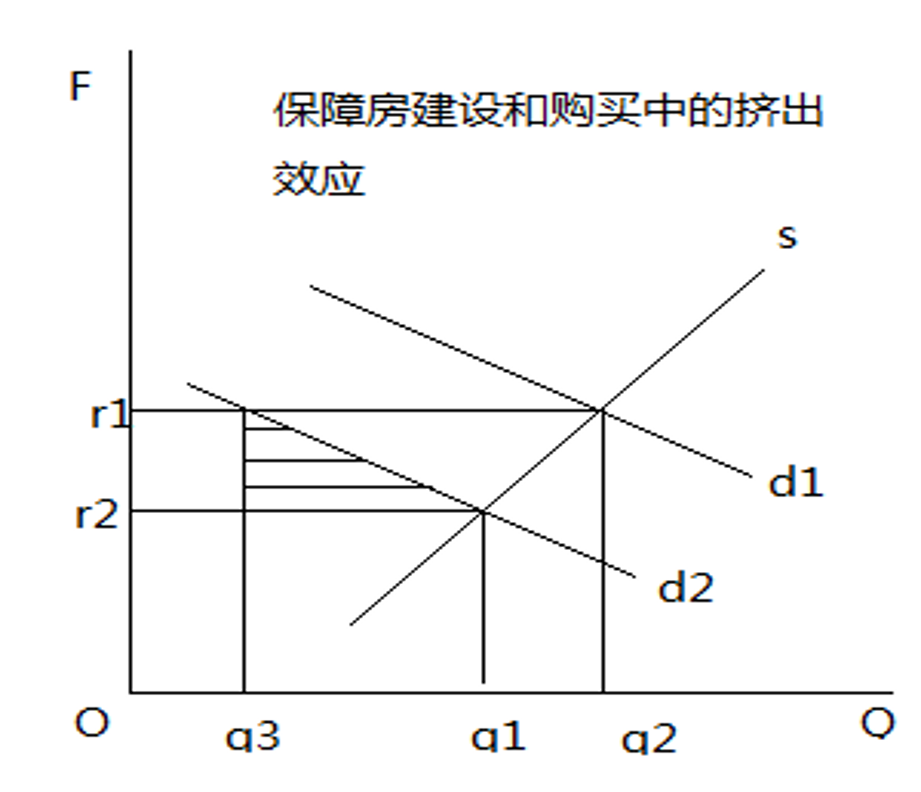
\includegraphics[width=1.0\textwidth]{./resources/figure/squeeze.png}
        \end{minipage}
        \end{figure}
\end{frame}

\begin{frame}[plain]
    \frametitle{(一)保障性住房建设环节的社会福利损失}
    在上图中由于开发商显性或隐性地改变保障房申购标准,一部分中高收入者加入到保障房需求行列中,从而使保障房需求曲线从d2上升到d1,在供给曲线不变的情况下,价格从r2上升到r1,图中阴影部分代表的一部分福利从中低收入者手中转移到中高收入者手中。依据福利经济学基数效用论的解释,这种社会福利从低收入者手中向中高收入者手中转移,必然降低社会总福利。
\end{frame}

\begin{frame}[plain]
    \frametitle{(二)保障性住房分配环节的社会福利损失}
    保障房针对中低收入“夹心层”这一定位本身便带有模糊性和调整定义的空间。若高收入者等强势群体介入保障房领域,则会对目标人群的福利甚至整个社会福利带来负面影响。根据公共经济学,保障房属于准公共产品,从各地保障房制度实践来看,保障房价格是周边同类同质商品房价格的70\%---80\%,甚至更低,这个准公共产品和纯私人商品之间的差价为“寻租”提供了空间。如下图所示:
\end{frame}

\begin{frame}[plain]
    \frametitle{(二)保障性住房分配环节的社会福利损失}
    \begin{figure}
        \centering
        \begin{minipage}{0.4\linewidth}
            在右图中供给曲线s和需求曲线d相交于点e,e代表均衡价格点,b是政府对保障房的限定价格,由于不同购房者的需求函数是有差异的,当保障房价格低于市场的均衡价格c时,消费者需求扩大,即一些在较高的均衡价格下原本不准备购房的人此时被纳入了有购房需求者的行列。
        \end{minipage}%
        \begin{minipage}{0.6\linewidth}
            \centering
            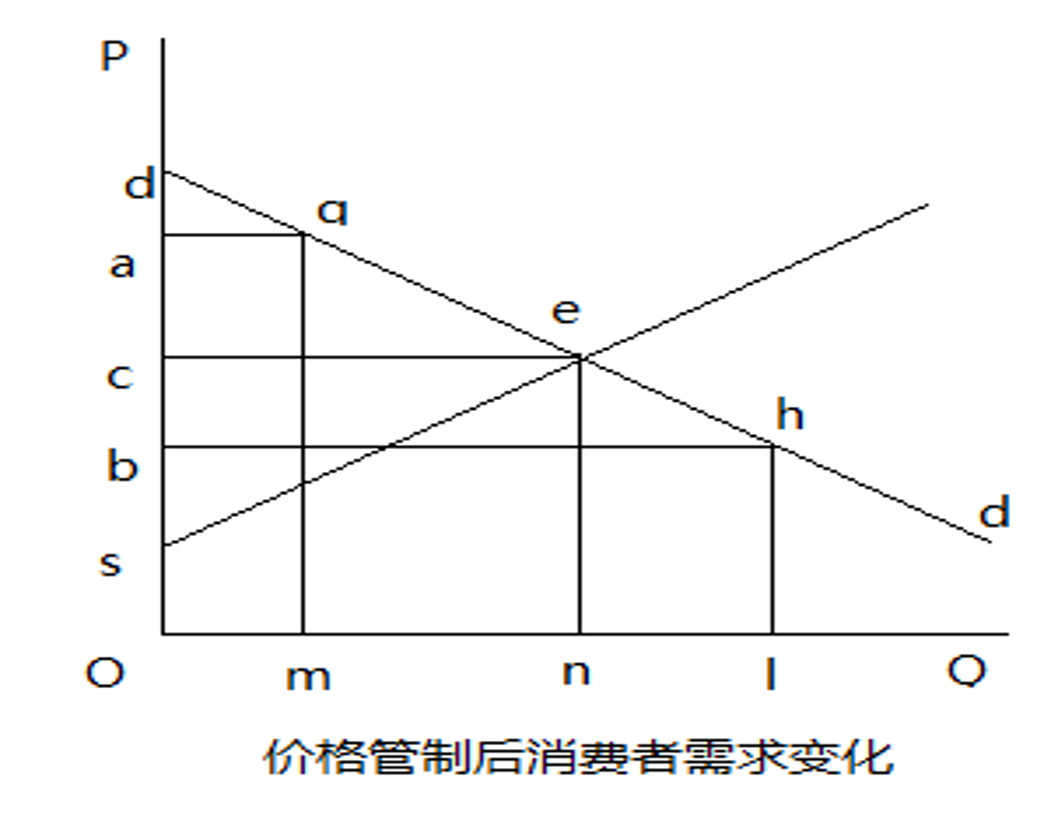
\includegraphics[width=1.0\textwidth]{./resources/figure/regulation.png}
        \end{minipage}
        \end{figure}
\end{frame}

\begin{frame}[plain]
    \frametitle{(二)保障性住房分配环节的社会福利损失}
    如果在市场决定的均衡价格下有能力购房的人没有被排除在保障房政策保障对象之外,或者采用其他手段加入到争购保障房者的行列,保障房的供给量就会相对萎缩。当存在保障房寻租空间时,由于关系网的差异,强势人群更容易在寻租的竞争中胜出,在一定程度上蚕食原本倾向于中低收入目标人群的福利资源。此外,为寻租所耗费的成本都不会形成生产力和实际财富,完全是无意义的资源耗费,是社会福利的净损失。
\end{frame}

\section{四、国外保障性住房制度的建设经验}

\begin{frame}[plain]
    \frametitle{(一)政府出台优惠政策保证保障房不以盈利为目的}
    新加坡政府在土地供应方面并非把市区的土地高价卖给私人发展商,而是通过划拨方式给建屋发展局兴建公共租屋,然后再以市场价二到三折的低价格出售给居民。
    \par
    香港政府因地制宜,根据时期特点制定相应的公屋计划,在通过低成本住房解决居民安置问题后,便督促开发商重视房屋质量,并及时考虑到保障房在市中心建设产生的负外部效应,开始实行“新市镇计划”。
    \par
    德国政府会向建设公共保障性住房的私人开发商提供财政补贴、无息贷款或税收优惠等政策,鼓励它们建造符合居住标准和价格相对合理的住房,建成后按照政府规定租金或价格标准进行出租或出售,不受市场价格变动的影响。
\end{frame}

\begin{frame}[plain]
    \frametitle{(二)建立严格、完善的抑制住房投机的法律法规}
    保障房涉及经济、社会、法律等多维度,单纯凭借单一力量无法完成,各国均通过完善相关立法,以规范、科学的程序审查申购者资格。
    \par
    日本政府在保障房建设方面出台了诸多法律以缓解住房压力,严格审查申购者资格,并成立专门的住房金融公库,对中低收入家庭发放低息长期的优惠贷款,而且还成立了专门的住房建设决策和管理监督部门——省住建局,通过强硬的行政手段督促各级部门履行公营住宅建设的义务。
\end{frame}

\begin{frame}[plain]
    \frametitle{(二)建立严格、完善的抑制住房投机的法律法规}
    美国在保障房监督方面除了制定相对完善的法律法规外,还邀请新闻媒体监督。
    \par
    德国政府制定详细的公共保障性住房退出规则,承租保障性住房的家庭,每年都必须向政府住房部门申报家庭收入,以确定是否具备保障性住房居住资格,凡收入超过规定标准的家庭应退还保障房,否则将按市场价格标准收取租金。
\end{frame}

\begin{frame}[plain]
    \frametitle{(三)多渠道拓宽保障房土地来源}
    英国保障性住房的土地来源有三个途径:
    \par
    第一,通过城市拆迁获得需要的建设用地,政府或受委托的市场主体对被拆迁群体进行赔偿,对其住房要求予以满足;
    \par
    第二,依据1890年《工人阶级住房法》可以接受社会各界所捐赠的土地、金钱及其他财务建设保障性住房;
    \par
    第三,英国设有贡献—义务机制,要求房地产商在获得房地产开发权的同时承诺向低收入者提供一定数量或者比例的经济适用房。
\end{frame}

\begin{frame}[plain]
    \frametitle{(三)多渠道拓宽保障房土地来源}
    美国政府对具体住房工程进行直接支持,以每年数十亿美元的投资,用于对旧住宅的修补,但很少对新住宅建设进行资助。
    \par
    瑞典在住房保障方面要求地方政府必须建立公众拥有的住房公司,通过公司参与住房建设的方式来推动住房数量的增长,并为所有来自农村的居民提供住房。
\end{frame}

\section{五、提升保障房制度社会福利效应的对策}

\begin{frame}[plain]
    \frametitle{(一)政府要加强规范房地产开发商的行为}
    首先,政府应减免保障性安居工程涉及的营业税、房产税、城镇土地使用税、土地增值税、印花税、契税等税收,降低保障性安居工程建设和营运的成本,在土地收益方面适当让利。
    \par
    其次,政府要强化土地审批制度的控制力度,从土地供应方面加强对房地产开发商的管理,规范其市场行为,并积极优化土地供应总量与结构,避免同区域在短时间内大幅度增加保障性住房供应量,导致供大于求、保障房空置的现象。
    \par
    第三,政府应要求房地产开发商针对保障性住房的实际需求情况合理开发适当的户型结构,增加小户型的供应量,避免出现较大户型。
    \par
    第四,加强对住宅建设的质量管理,合理选址并完善公共设施配套。
\end{frame}

\begin{frame}[plain]
    \frametitle{(二)完善保障房的准入准出和社会监督机制}
    首先,要建立严格的保障房准入条件。保障房制度的准入指标应包含家庭收入水平、家庭资产以及现有住房条件,并在保障房的申报、审核、公示中详细列举准入条件和申请者的基本情况。
    \par
    其次,健全保障房准出机制。当保障对象的收入水平超出保障标准后,要求其主动申报退还保障房;政府部门提供必要的退出渠道。
\end{frame}

\begin{frame}[plain]
    \frametitle{(二)完善保障房的准入准出和社会监督机制}
    第三,建立保障房的社会监督机制。采取专门的保障分配管理措施:
    \par
    1.制定具体的轮候管理制度以防范分配过程中出现的不公现象;
    \par
    2.坚持分配中的公开性原则,制定具体的措施和惩罚办法以最大程度杜绝徇私舞弊现象;
    \par
    3.建立规范的信息披露和公示制度,将保障房的分配过程暴露在公众监督之下,加强保障房科学化、规范化管理。
\end{frame}

\begin{frame}[plain]
    \frametitle{(三)积极拓宽保障房的房源渠道}
    一是继续加大新建保障房的建设规模;
    \par
    二是政府出资收购符合基本住房标准的存量房,收购原则是配套设施齐全、交通便捷、价格适中、小户型为主的二手住房和普通商品房;
    \par
    三是将财政投资建设的单位自管公房房源纳入保障房房源管理;
    \par
    四是鼓励单位、社会、个人捐增闲置房屋,并鼓励符合条件的私人房屋拥有者出租住房,作为保障房房源补充;
    \par
    五是政府建立保障房回购制度,帮助一些已购买保障房但因各种原因无力供楼的家庭减轻压力,避免违规事件的发生;
    \par
    六是逐步建立保障房的二级市场,允许保障房在符合条件的前提下,在二级市场中进行交易,加大中低收入群体的购房自由度,减少等候时间。
\end{frame}

% ---------------------------------------------------------------------------
\begin{frame}[standout]
    \begin{center}
        {\Huge\calligra Thanks!}
      \end{center}
\end{frame}
% ---------------------------------------------------------------------------

\end{document}
